\documentclass[a4paper]{article}
\usepackage[top=19mm, bottom=43mm, right = 14.32mm, left = 14.32mm]{geometry}

\usepackage{float}
\usepackage{graphicx}
\usepackage{wrapfig}
\usepackage[shortlabels]{enumitem}


\usepackage{multicol,caption}

\usepackage[T1]{fontenc}
\usepackage{mathptmx}
\begin{document}
\pagenumbering{gobble} 
\newpage

\begin{center}
{\fontsize{24pt}{28.8pt}\selectfont A Deep Dissertion of Data Science: Related
Issues and its Applications}
 
\end{center}

\begin{center}
\textbf{Sanyukta Shreshtha$^{1}$, Archana Singh$^{2}$, Sanya Sahdev$^{3}$, Millennium Singha$^{4}$, Siddharth Rajput$^{5}$}
\end{center}

	\begin{center}
	\textit{$^{1,2,3,4,5}$Department of Information Technology, ASET, Amity University Uttar Pradesh, NOIDA\\
	$^{1}$sanyuktashreshtha2000@gmail.com, $^{2}				$archana.elina@gmail.com
	$^{3}$sanya.sahdev2204@gmail.com, $^{4}					$millenniums909@gmail.com, $^{5}$sidd7399@gmail.com}
\end{center}
\hrule
\vspace{10pt}

  
\begin{multicols}{2}
\noindent \textit{\textbf{Abstract: Data Science refers to a study of extracting,
collection, gathering data, representing and protecting data
to be used for business purposes or in technical issues.
Despite the fact that the name Data Science appears like
something which meant, databases and software engineering,
various types of quantitative and qualitative aptitudes
including nonmathematical abilities are additionally required
here. Data Science is mainly breaking down information.
This paper illustrates What is Data Science, How it
processes, and also its Applications. Section II of this paper
consists of the different review regarding data science.
Section III of this paper illustrates about the complete
process of data science. Section IV describes all the related
research issues for data science. At the end the paper is
concluded with some suggested future work regarding data
science. In the present paper the authors will attempt to
investigate the diverse issues, execution and difficulties in
territory called Data science. \\ \\
Keywords: Information, Data Science, investigation,
management, cloud computing.}}

\subsection*{I. INTRODUCTION}
Data Science is the accumulation from substantial volume of
data that are merged or free, or, in other words of the field of
data scooping and perceiving research, by and large called data
disclosure and data mining. John Tukey's announcement this
topic and the conclusion he made is: "The mix of a couple of
data and a throbbing need for an answer does not ensure that a
sensible answer can be isolated from a given collection of
data". \\ \\
To QuoteHal Varian, Google'sEconomist, "The capacity to
take information—to have the capacity to comprehend it, to
process it, to remove an incentive from it, to imagine it, to
convey it—that will be a gigantically essential expertise in the
following decades. Since now we truly do have basically free
and omnipresent information. So the complimentary rare factor
is the capacity to comprehend that information and concentrate
an incentive from it”. The field of this science includes data
sequencing, collecting and presenting, bits of knowledge, and
machines presuming out with how to deal with different issues
in different field.

\subsection*{II. LITERARY REVIEW}
Dr.S.Justus (2013), outlined that the capacity and recovery
frameworks, the entrance layers and procedures for Big Data
are advancing step by step. Test Architects and Testing groups
are not barred in this big situation. They centres around a
portion of the difficulties test groups would look soon. J.
Nowling (2014), delineated that generating a lot of
semantically-rich data for testing big data workflows is vital
for adaptable execution benchmarking and quality affirmation
in current machine-learning and examination outstanding tasks
at hand. Brucke, Volker Markl (2013), represented that the
scholarly network and industry are at present exploring and
working cutting edge data administration frameworks. These
frameworks are intended to examine data sets of high volume
with high data ingest rates. C. L. Philip Chen (2014) expressed
that another coherent perspective is considered as data serious
intelligent revelation (DISD), generally called Big Data issues.
A sweeping number of fields and portions, running from
monetary and business activities to open association, from
national security to consistent investigates in various domains,
incorporate with Big Data issues.

\subsection*{III. DATA SCIENCE PROCESS}
\noindent 
    \begin{minipage}{\linewidth}
      \centering
      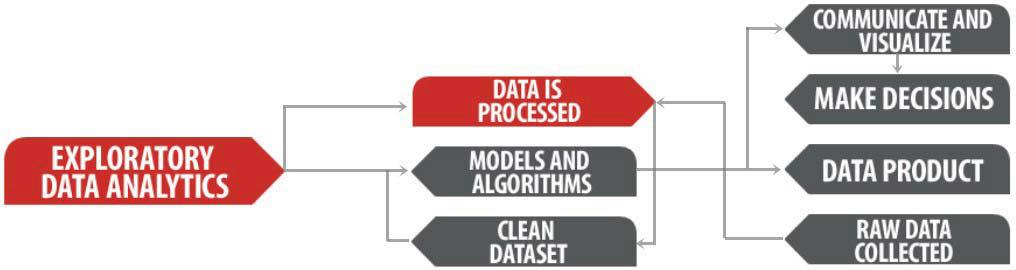
\includegraphics[width= 8cm]{fig1}
      \captionof*{figure}{\textbf{Fig. 1. Steps Invloved in A Data Science Process}}
    \end{minipage}


\vspace{10pt}
The three pieces fused into data science are organizing,
assembling and passing on data (the ABC of data). At any rate
assembling is an imperative snippet of data wrangling, which
consolidates assembling and orchestrating of data. In other
words it’s like what limits data science from other different
issues is the awareness that what, why, how. A data specialist
needs to fundamentally accept who the general population are
that will be joined into making the profit. Following are the
channels associated with a data science process.  \\

\textit{1. Data wrangling and transforming:\\ }
Converting data into another format is called data wrangling.
Get-together data from material zones and the system of
physically changing over or mapping data from one "rough"
shape into another association that considers more favourable
use is known as data wrangling or transforming. Instigating
advances and limits is the substance of change. Shoving data is
the ensuing stage that seeks after orchestrating data. Shoving
data fuses dependably controlling and joining the essential
unpleasant data into another depiction and bundle. Shoving
data is extremely the backwards of managing data and fuses
moving as one.
\\ \\
\textit{2. Data Investigation:\\}
Examination of data is a route of evaluating, transforming, and
presenting data with the objective of exploring pleasing data
and accompanying fundamental authority. The data is readied
through diverse counts of bits of knowledge and machine
making sense of how to expel importance and profitable
finishes from the broad volumes of data. \\ \\
\textit{3. Transfer Data: \\}
Transferring data fuses systems to change the numerical or
quantifiable finishes taken from the facts into an edge that can
be adequately grasped and deciphered by analyst requiring it.
Exchanging Data is permitting the change starting with one
perspective then against the accompanying.

\subsection*{IV. OPEN RESEARCH ISSUES FOR DATA SCIENCE}
Data science is transmuting into the inspection purpose of
combination in endeavours and the insightful world. Data
science undergoes investigating immense data and comprising
extraction from the data. The investigation issues identifying
with gigantic data examination are organized into three general
classes particularly internet of things (IoT), cloud computing
and quantum computing. In any case it isn't obliged to such
problems. \\
\end{multicols}

\begin{figure}[h]
\begin{center}
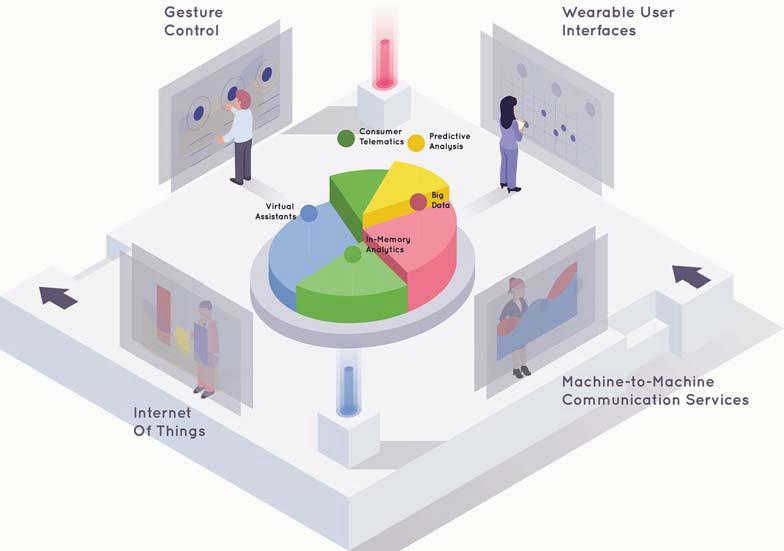
\includegraphics[width = 0.75\textwidth]{fig2}
\caption*{\textbf{Fig. 2. Pie Chart of Emerging Technologies in Data Science}}
\end{center}
\end{figure}

\begin{multicols}{2}
\textit{1. IoT for Data Science:\\}
By and by, machines are getting in on the exhibit to control
endless autonomous gadgets by methods for web and make
Internet of Things (IoT). In this manner, mechanical
assemblies are transforming into the customer of the web,
much the equivalent as individuals with the web programs.
Internet of Things is attracting the thought of investigators for
its most promising possibilities and troubles. It has an essential
financial and societal impact for the future improvement of
data, framework and correspondence development. The new
bearing of future will be over the long haul, everything will be
related and wisely controlled. The possibility of IoT is winding
up more important to the sensible world on account of the
headway of phones, rooted and all inclusive correspondence
developments, conveyed figuring, and data examination. IoT
these days wind up significant research issue among analysts. \\

\textit{2. Cloud Computing for Data Science:\\}
Computing frameworks that are covered up in virtualization
programming make frameworks to act like a genuine PC, yet
with the adaptability of particular points of interest, for
example, processors, plate space, memory, and working
framework. Enormous Data and cloud computing
advancements are produced with the significance of building
up a versatile and on interest accessibility of assets and
information. Cloud computing orchestrate enormous
information by onmandate access to organizable figuring
assets through cybernetic procedures. The advantages of using
the Cloud computing incorporate recommending assets when
there is an interest and pay just for the assets which is expected
to build up the item. \\ \\
\textit{3. Quantum Computing for Data Science:\\}
If a bona fide quantum PC is open now, it could have handled
issues that are exceptionally troublesome on continuous PCs,
clearly the present immense data issues. The standard specific
inconvenience in building quantum PC could after a short time
be possible. Quantum figuring gives a way to deal with
consolidate the quantum mechanics to process the data.
Likewise, it has a tendency to be picked up by the miracles of
different parts and capture. It is by virtue of qubits act quantumly.

\subsection*{V. APPLICATIONS OF DATA SCIENCE}
Data science is a subject that emerged principally from need,
with regards to genuine applications rather than as an
exploration area. Throughout the years, it has developed from
being utilized in the moderately tight field of measurements
and investigation to being an inclusive nearness in every aspect
of science and industry. In this segment, we take a gander at a
portion of the central territories of utilizations and research
where data science is presently utilized and is at the cutting
edge of advancement. \\ \\
Business Analytics – Collecting information about the various
times execution of a business can give understanding into the
working of the business and help drive basic leadership
procedures and construct prescient models to figure future
execution. A few researchers have contended that information
science is simply another word for business analytics, which
was a transiently rising field a couple of year back, just to be
supplanted by the new trendy expression information science.
Regardless of whether the two fields can be thought to be
commonly free, there is almost certainly that information
science is in all inclusive use in the field of business
examination.

\begin{enumerate}
\item Expectation – Large proportions of data accumulated and
separated can be used to identify outlines in data, which
can consequently be used to gather perceptive models.
This is the preface of the field of machine acknowledging,
where data is acknowledgment figuring and on various estimations that are said to "learn". Machine learning
strategies are, all things considered, used to develop
perceptive models in different fields.

\item Security – Facts collected from analyst logs are utilized to
recognize fraud utilizing information science. Examples
distinguished in client action can be utilized to disconnect
instances of extortion and malignant insiders. Banks and
other monetary predominantly utilize information mining
and machine learning calculations to counteract instances
of fraud.

\item Computer Vision – Data from picture and video
investigation is utilized to execute PC vision, which is the
study of making PCs "see", utilizing picture information
and learning calculations to gain and break down pictures
and take choices in like manner. This is utilized in apply
autonomy, self-sufficient vehicles and human-PC
cooperation applications.

\item Natural Language Processing – Modern NLP methods
utilize tremendous measures of literary information from
corpora of records to factually show etymological
information, and utilize these models to accomplish
undertakings like machine translation, parsing,
characteristics dialect age and notion analysis.
\end{enumerate}
 
\noindent 
    \begin{minipage}{\linewidth}
      \centering
      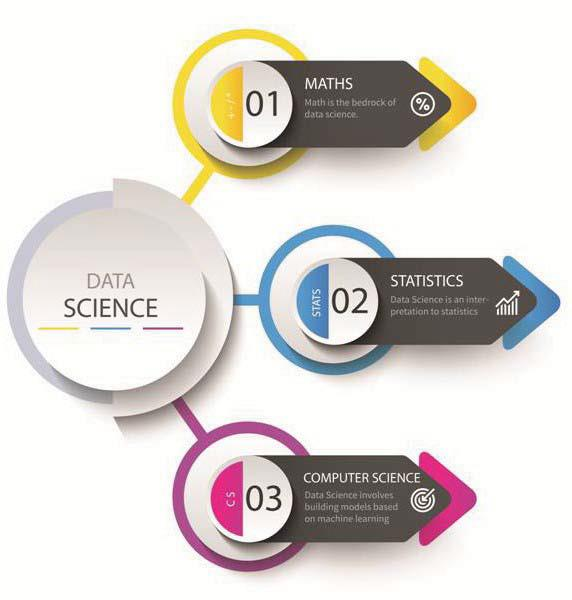
\includegraphics[width= 8cm]{fig3}
      \captionof*{figure}{\textbf{Fig. 3. Data Science Model}}
    \end{minipage}
\vspace{5pt}
\subsection*{VI. SUGGESTIONS FOR FUTURE WORK}
The amount of information gathered from different
applications everywhere throughout the world over a wide
assortment of fields today is relied upon to twofold at regular
intervals. It has no utility except if these are investigated to get
942
valuable data. This requires the improvement of methods
which can be utilized to encourage huge information
investigation. The advancement of great PCs is an aid to
execute these methods prompting mechanized frameworks.
The change of information into learning is in no way, shape or
form a simple undertaking for elite extensive scale information
handling, including misusing parallelism of present and up and
coming PC models for data mining. \\ \\
Frequently the data gathered have missing qualities. All the
more critically, these new difficulties may involve, once in a
while even decay, the execution, effectiveness and adaptability
of the information concentrated processing frameworks.
Furthermore, quick preparing while at the same time
accomplishing superior and high throughput, and putting away
it productively for later is another issue. The effective
instruments to be created must have arrangement to deal with
boisterous and unevenness information, vulnerability and
irregularity, and missing qualities. 

\subsection*{VII. CONCLUSION}
In late year, data are made at an incredible pace. To this end in
this paper, we audit the diverse research issues, challenges, and
applications identified with data science. From this overview,
it is comprehended that each enormous information stage has
its individual core interest. Some of them are intended for
bunch preparing while some are great at constant investigative.
Each huge information stage additionally has particular
usefulness. Distinctive methods utilized for the investigation
incorporate factual examination, machine learning, information
mining, insightful examination, distributed computing,
quantum registering, and information stream handling. We
belive that in future analysts will give careful consideration to
these methods to take care of issues of enormous information
successfully and effectively.

\begin{thebibliography}{} 
\bibitem "Big Data: The Next Frontier for Innovation Competition and
Productivity" in McKinsey Global Institute, 2011.

\bibitem B. F. Jones, S. Wuchty, B. Uzzi (2008), in "Multi-University
Research Teams: Shifting Impact Geography and Stratification
in Science", Science 322, pp. 1259-1262.

\bibitem C. L. Philip, Q. Chen and C. Y. Zhang (2014), inData-intensive
applications, challenges, techniques and technologies: A survey 
on big data, Information Sciences, 275, pp.314-347.

%\bibitem $ https://en.wikipedia.org/wiki/Data_science. $

\bibitem J. Dean, S. Ghemawat, Jan (2008), in "MapReduce: Simplified
data processing on large clusters", Commun. ACM, vol. 51, no.
1, pp. 107-113

\bibitem J. Manyika, B. Brown, J. Bughin, R. Dobbs, C. Roxburgh, A.
Byers (2011), from Big data: The Next Frontier for Innovation
Competition and Productivity.
\bibitem M. Armbrust, A. Fox, R. Griffith, A. D. Joseph, A. Konwinski,
G. Lee, D. Patterson, A. Rabkin, I. Stoica, M. Zaharia, Apr
(2010), "A view of cloud computing", Commun. ACM, vol. 53,
no. 4, pp. 50-58.

\bibitem M. Hilbert, P. Lopez (2011), from "The world’s technological
capacity to store communicate and compute information",
Science, vol. 332, no. 6025, pp. 60-65.

\bibitem M. K.Kakhani, S. Kakhani and S. R.Biradar (2015), Research issues in big data analytics, International Journal of Application or Innovation in Engineering and Management, 2(8), pp.228-232.

\bibitem M. M. Waldrop (1992), "Complexity: The Emerging Science at the Edge of Order and Chaos", Simon and Schuster.

\bibitem P. Chapman, J. Clinton, R. Kerber, C. Shearer, R. Wirth (2000),
in "CRISP-DM 1.0: Step-by-step data mining guide", The
CRISP-DM Consortium.

\bibitem S. Wuchty, B. F. Jones, B. Uzzi (2007), "The Increasing
Dominance of Teams in Production of Knowledge", Science
316, pp. 1038-1039.

\bibitem T. H. Davenport, J. G. Harris (2007), Competing on Analytics:
The New Science of Winning, Harvard Business School Press.

\bibitem W. v.d. Aalst (2011), Process Mining: Discovery Conformance
and Enhancement of Business Processes, Berlin, Germany:
Springer-Verlag.
\end{thebibliography} 
\end{multicols}


\end{document}
